\subsection{Experiment 6: Optimizing Model Balance} \label{sec:exp6}

In this experiment, the author aimed to leverage the upgraded hardware configuration of the \ac{LIACC} 2 system. After updating the model to include the Clotho dataset, which demanded more significant \ac{GPU} and \ac{RAM} resources, the results were analyzed.

Nevertheless, the author found them unsatisfactory, possibly due to the imbalance of the generator and discriminator models, with the former having about 25 million parameters and the latter having only about 2 million. Typically, \ac{GAN} models are designed as a pair of similar or mirrored models.

To mitigate this problem, the author reversed the model difference that was introduced in Experiment 3. The generator and discriminator models were both adjusted to have around 2 million parameters each.

The loss function, regularization techniques, and optimizer remained unchanged. The total loss for this experiment was $2.045$, calculated by adding the generator loss of $0.587$ and the discriminator loss of $1.458$.

For a visual representation of the results, which includes the loss and the final spectrogram generated in this experiment, please see Figure~\ref{fig:exp6_results}.

\begin{figure}[!ht]
    \centering
    \begin{subfigure}{0.45\textwidth}
        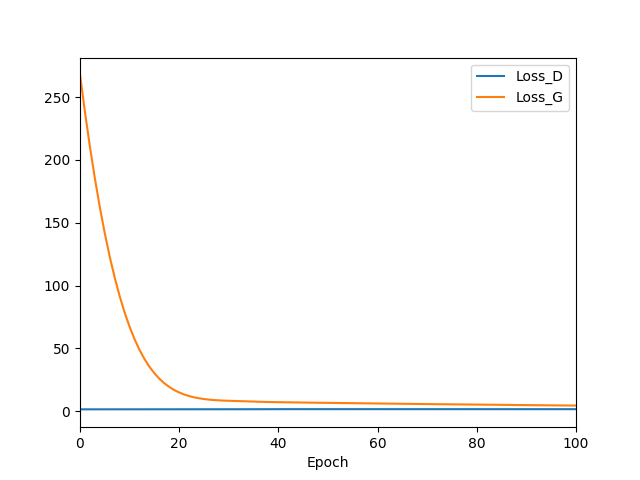
\includegraphics[width=\textwidth]{figures/4.5-results/exp6_loss.png}
        \caption{Evolving losses throughout the training process for Experiment 6.}
        \label{fig:exp6_loss}
    \end{subfigure}
    \begin{subfigure}{0.45\textwidth}
        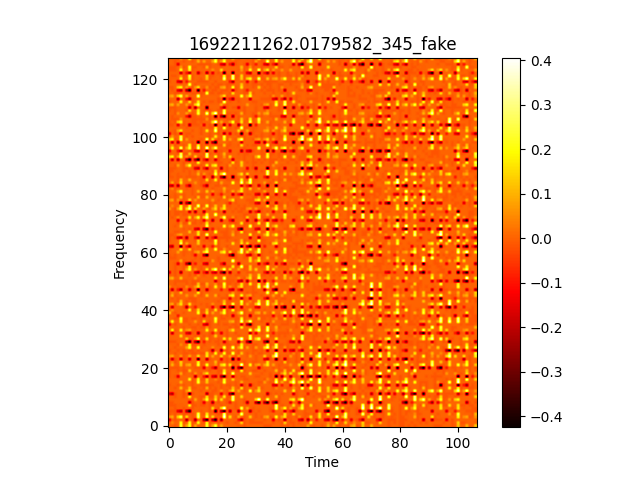
\includegraphics[width=\textwidth]{figures/4.5-results/exp6_spectrogram.png}
        \caption{Spectrogram generated in Experiment 6.}
        \label{fig:exp6_spectrogram}
    \end{subfigure}
    \caption{Results of Experiment 6.}
    \label{fig:exp6_results}
\end{figure}